\documentclass[UTF8]{ctexrep}

\usepackage{graphicx}

\ctexset{
    section/name = {第,节},
    section/number = {\arabic{section}},
    subsection/number = {\arabic{section}.\arabic{subsection}}
}

\title{Aminer调研报告}
\author{王清雨}
% \usepackage{apacite}
\bibliographystyle{acm}

\begin{document}

\maketitle
\newpage
\part{历史}
\section{aminer发展历史}

\paragraph{2006年6月}
信息提取,学者、论文、会议搜索
\paragraph{2006年8月}
重写上述功能
\paragraph{2007年7月}
添加学者研究兴趣、关联搜索(\textbf{\textit{association search}})、\textbf{\textit{survey search}}?
\paragraph{2008年4月}
查询理解(\textbf{\textit{Query understanding}})、新的搜索界面、日志分析
\paragraph{2008年11月}
图搜索、主题挖掘(\textbf{\textit{topic mining}})
\paragraph{2009年4月}
信息编辑、开放资源
\paragraph{2009年12月}
学术统计数据(\textbf{\textit{Academic statistics}})、用户反馈、精细化排名

\section{论文发表历史}

\subsection{社交网络分析}
\textbf{\textit{Topic-based} social influence analysis in large-scale networks}

%--------------------------%

\paragraph{2009年}
\subparagraph{Social influence analysis in large-scale networks}~\cite{tang2009social}
\par 主要研究社交网络\textbf{\textit{(social network)}}的建模、分类及其内部关系,提出了\textbf{Topical Affinity Propagation}用来对社交网络进行建模。最终能够找到一个topic下最具代表性的节点,同时发现节点对周围节点的影响。
\par 有很多看不懂的机器学习的公式和算法

\subparagraph{Topic distributions over links on web}~\cite{tang2009topic}
\par 主要研究如何对网页上的链接进行分类和如何量化链接的影响力
\par 接下来就看不懂了

\begin{figure}[h]
    \caption{topical factor graph model}
    \centering
    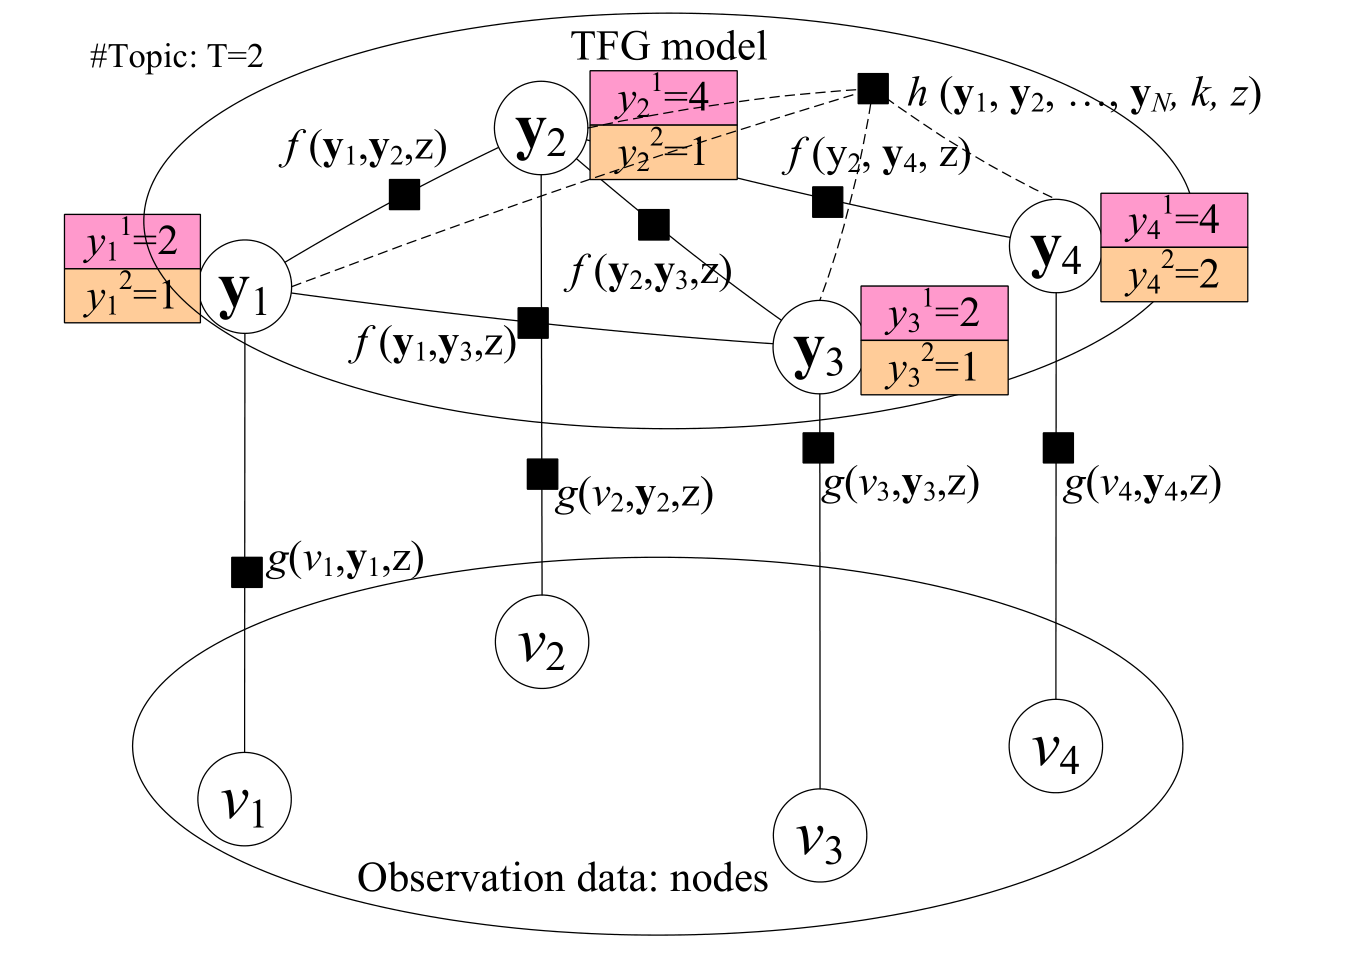
\includegraphics[width=0.8\textwidth]{assets/figures/model1.png}
    \label{fig:model1}
\end{figure}
%--------------------------%

\paragraph{2010年}
\subparagraph{Mining Advisor-Advisee Relationships from Research
Publication Networks}\cite{wang2010mining}
\par 主要研究如何将导师、学生关系从合作关系中提取、挖掘出来,并给出一种学习方法,用来提升提取的效果。

\par 可见这是如今\texttt{aminer}\footnote{https://www.aminer.cn}所做的事情的简化版。
\par {\heiti 关键词:}\emph{relationship mining, time-constrained probabilistic factor graph model, jointly likelihood objective function, advisor-advisee prediction}


\subparagraph{论文3~\cite{yang2010social}}
\subparagraph{Social community analysis via a factor graph model}~\cite{tan2010social}
\par 与\cite{tang2009topic}基本相同


%--------------------------%

\subsection{社交网络排名}
\textbf{Topic-based heterogeneous ranking}

\paragraph{2008年}
\subparagraph{论文\cite{tang2008topic}}
\subparagraph{论文\cite{tang2008arnetminer}}

%--------------------------%

\subsection{知识获取}
\textbf{Acquiring knowledge from social Web}

\paragraph{2006年}
\subparagraph{论文\cite{tang2006tree}}

\paragraph{2007年}
\subparagraph{论文\cite{tang2007social}}
\subparagraph{论文 \cite{zhang2007constraint}}

\paragraph{2010年}
\subparagraph{论文\cite{tang2010combination}}


3~\cite{tang2011unified}
\newline
4~\cite{wang2011adana}
\newline
5~\cite{zhang2018name}


\part{组织结构}

\part{特点}
\part{后台技术}

\bibliography{papers}
\end{document}
